\documentclass[SKL-MASTER.tex]{subfiles}
\begin{document}
	\LARGE
	\noindent \textbf{Logistic Regression}\\
	Linear models can actually be used for classification tasks. This involves fitting a linear model
	to the probability of a certain class, and then using a function to create a threshold at which
	we specify the outcome of one of the classes. \\ 
	
	\bigskip
% %	\subsubsection{Getting ready}\\
	\noindent \textbf{The Logistic Function}\\
	The function used here is typically the logistic function. The logistic function $f(t)$ is defined as follows:
	\[ f (t) = \frac{e^t}{e^t+1} = \frac{1}{1+e^{-t}},\]
	%========================================================%
	% % Working with Linear Models
	% % 76
	\bigskip
	Visually, it looks like the following:
	\begin{figure}[h!]
		\centering
		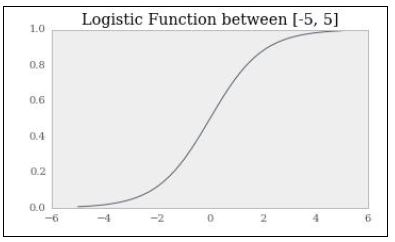
\includegraphics[width=0.7\linewidth]{LogisticFunctions}
		% \caption{}
		% \label{fig:LogisticFunctions}
	\end{figure}\\ 
	Here the range of values is $[-5,5]$, the transition region. In practice most values of $t$ will be outside this region.
	
	\[ f (8) = \frac{1}{1+e^{-8}} = \frac{1}{1+0.00034} = 0.99966 \approx 1 \]
	
	\newpage
	\subsection*{Worked Example : Create some Data}
	Let's use the \texttt{make\_classification} method, create a dataset. We will have 1000 cases with 4 features. This data is contained in $X$. The targets are 0s and 1s , contained in $Y$.
	{
		\large
		\begin{framed}
			
			\begin{verbatim}
			>>> from sklearn.datasets import make_classification
			>>> X, y = make_classification(n_samples=1000, n_features=4)
			\end{verbatim}
		\end{framed}
	}
	\subsection*{Implementation}
	The \texttt{LogisticRegression} object works in the same way as the other linear models:
	{
		\large
		\begin{framed}
			\begin{verbatim}
			>>> from sklearn.linear_model import LogisticRegression
			>>> lr = LogisticRegression()
			\end{verbatim}
		\end{framed}
	}
	\noindent Here we have an ``empty" model called \texttt{lr}, ready to be trained.
	\subsection*{Splitting the Data Set}
	\begin{itemize}
		\item We will use the last 200 samples to test the trained
		model on. 
		\item Since this is a random dataset, it's fine to hold out the last 200.
		\item If you're dealing
		with structured data, don't do this (\textit{for example, if you deal with time series data}):
	\end{itemize}
	
	\begin{framed}
		\begin{verbatim}
		>>> X_train = X[:-200]
		>>> X_test = X[-200:]
		>>> y_train = y[:-200]
		>>> y_test = y[-200:]
		\end{verbatim}
	\end{framed}
	% We'll discuss more on cross-validation later in the book. 
	\begin{itemize} 
	\item Now, we need to fit the model with
logistic regression. 
\item We can use the trained model to make predictions on both the testing data set, and the training data set.
% We'll keep around the predictions made on the train set, just like the test set. It's
%	a good idea to see how often you are correct on both sets.
\item Remark: Often, you'll be better on the train set; it's a matter of how much worse you are on the test set:
\end{itemize}	
	\begin{framed}
		\begin{verbatim}
		>>> #  Train the Model
		>>> lr.fit(X_train, y_train)
		>>>
		>>> # Lets try it out
		>>> y_test_pred = lr.predict(X_test)
		>>> y_train_pred = lr.predict(X_train)
	
		\end{verbatim}
	\end{framed}
	%========================================================%
	% % Chapter 2
	% % 77
	\newpage
	\noindent \textbf{Model Evaluation}\\
	\begin{itemize}
		\item Now that we have the predictions, let's take a look at how good our predictions were. 
		\item Here,
		we'll simply look at the number of times we were correct.
		% \item ; later, we'll talk about evaluating classification models in more detail.
		\item The calculation is simple; it's the number of times we were correct over the total sample:
	\end{itemize}
	
	{
		\Large
		\begin{framed}
			\begin{verbatim}
			>>> # Number of Cases
			>>> y_train.shape[0]
					1000
				
						>>> (y_train_pred == y_train).sum().astype(float)/1000
			
				0.8662499
			>>> # 86.6 % success rate on training data
			\end{verbatim}
		\end{framed}
	}
	\noindent Similarly for the test sample:
	{
		\Large
		\begin{framed}
			\begin{verbatim}
			>>> (y_test_pred == y_test).sum().astype(float) / 1000
			
			0.900000
				>>> # 90 % success rate on training data
			\end{verbatim}
		\end{framed}
	}
	% So, here we were correct about as often in the test set as we were in the train set. Sadly, in
	% practice, this isn't often the case.
\newpage
	\subsection*{Class Imbalance}
	\begin{itemize}
		
		\item There will be a situation where one class is weighted differently
		from the other classes; for example, one class may be 99 percent of cases. 
		\item This situation will occur regularly in real world data science. 
		\item The canonical example is fraud detection,
		where most transactions aren't fraud, but the cost associated with misclassification is
		asymmetric between classes.
	\end{itemize}
	\newpage
	
	\noindent Let's create a classification problem with 95 percent imbalance and see how the basic stock
	logistic regression handles this case:
	
	
	%========================================================%
	% % Working with Linear Models
	% % 78
	\begin{framed}
		\begin{verbatim}
		>>> X, y = make_classification(n_samples=5000, 
		n_features=4,
		weights=[.95])
		>>>
		>>>  #to confirm the class imbalance
		>>> sum(y) / (len(y)*1.)
		0.0555
		\end{verbatim}
	\end{framed}
	
	\noindent Create the train and test sets, and then fit logistic regression:
	\begin{framed}
		\begin{verbatim}
		>>> X_train = X[:-500]
		>>> X_test = X[-500:]
		>>> y_train = y[:-500]
		>>> y_test = y[-500:]
		>>>
		>>> lr.fit(X_train, y_train)
		>>> y_train_pred = lr.predict(X_train)
		>>> y_test_pred = lr.predict(X_test)
		\end{verbatim}
	\end{framed}
	\newpage
\noindent	Now, to see how well our model fits the data, do the following:
	{
		\large
		\begin{framed}
			\begin{verbatim}
			
			>>> (y_train_pred == y_train).sum().astype(float) / y_train.shape[0]
			
			0.96977
			>>> (y_test_pred== y_test).sum().astype(float) / y_test.shape[0]
			
			0.97999
			\end{verbatim}
		\end{framed}
	}
	\begin{itemize}
		\item At first, it looks like we did well, but it turns out that when we always guessed that a transaction
		was not fraud (or class 0 in general) we were right around 95 percent of the time. 
		\item If we look at
		how well we did in classifying the 1 class, it's not nearly as good:
	\end{itemize}
	
	{
		\Large
		\begin{framed}
			\begin{verbatim}
			>>> (y_test[y_test==1] == y_test_pred[y_test==1])
			.sum().astype(float) / y_test[y_test==1].shape[0]
			
			0.583333
			\end{verbatim}
		\end{framed}
	}
	\newpage
	\begin{itemize}
		\item Hypothetically, we might care more about identifying fraud cases than non-fraud cases;
		this could be due to a business rule, so we might alter how we weigh the correct and
		incorrect values.
		\item By default, the classes are weighted (and thus resampled) in accordance with the inverse
		of the class weights of the training set. However, because we care more about fraud cases,
		let's oversample the fraud relative to nonfraud cases.
		\item We know that our relative weighting right now is 95 percent nonfraud; let's change this to
		overweight fraud cases:
	\end{itemize}
	{
		\Large
		\begin{framed}
			\begin{verbatim}
			
			>>> lr = LogisticRegression(class_weight={0:.15, 1:.85})
			>>> lr.fit(X_train, y_train)
			\end{verbatim}
		\end{framed}
	}
	\newpage
	Let's predict the outputs again:
	{
		\Large
		\begin{framed}
			\begin{verbatim}
			
			>>> y_train_pred = lr.predict(X_train)
			>>> y_test_pred = lr.predict(X_test)
			\end{verbatim}
		\end{framed}
	}
	%========================================================%
	% % Chapter 2
	% % 79
	\noindent We can see that we did a much better job on classifying the fraud cases:
	{\Large
		\begin{framed}
			\begin{verbatim}
			>>> (y_test[y_test==1] == y_test_pred[y_test==1]).sum().
			astype(float) / y_test[y_test==1].shape[0]
			0.875
			\end{verbatim}
		\end{framed}
	}
	\noindent At what expense do we do this? To find out, use the following command:
	{\Large
		\begin{framed}
			\begin{verbatim}
			>>> (y_test_pred == y_test).sum().astype(float) / y_test.shape[0]
			0.967999
			\end{verbatim}
		\end{framed}
	}
	
	\begin{itemize}
		\item Here, there's only about 1 percent less accuracy. Whether thatis acceptable  depends on your
		problem. 
		\item Put in the context of the problem, if the estimated cost associated with fraud
		is sufficiently large, it can eclipse the cost associated with tracking fraud.
	\end{itemize}
		\newpage
		\noindent \textbf{Skip This}
		\begin{itemize}
			\item The question then changes to how to move on from the logistic function to a method by which
			we can classify groups.
			\item First, recall the linear regression hopes offending the linear function that fits the expected
			value of Y, given the values of X; this is $E(Y|X) = X\beta$. Here, the Y values are the probabilities
			of the classes. 
			\item Therefore, the problem we're trying to solve is $E(p|X) = X \beta$. Then, once the
			threshold is applied, this becomes $\mbox{Logit}(p) = X\beta$. 
			\item The idea expanded is how other forms of
			regression work, for example, Poisson.
		\end{itemize}
		\newpage
\end{document}